% 2D Image with indices
% Author: Peter Steinbach
\documentclass[tikz]{standalone}
%\documentclass[dvisvgm]{standalone}
%\def\pgfsysdriver{pgfsys-tex4ht.def}
\usepackage{units}
\usepackage{tikz}
\usetikzlibrary{calc,trees,positioning,arrows.meta,chains,shapes.geometric,shapes.arrows,%
    decorations.pathreplacing,decorations.pathmorphing,shapes,%
    matrix,shapes.symbols,fit,backgrounds}

 \pgfdeclarelayer{back}
 \pgfsetlayers{background,back,main}


\makeatletter
\makeatother

\begin{document}
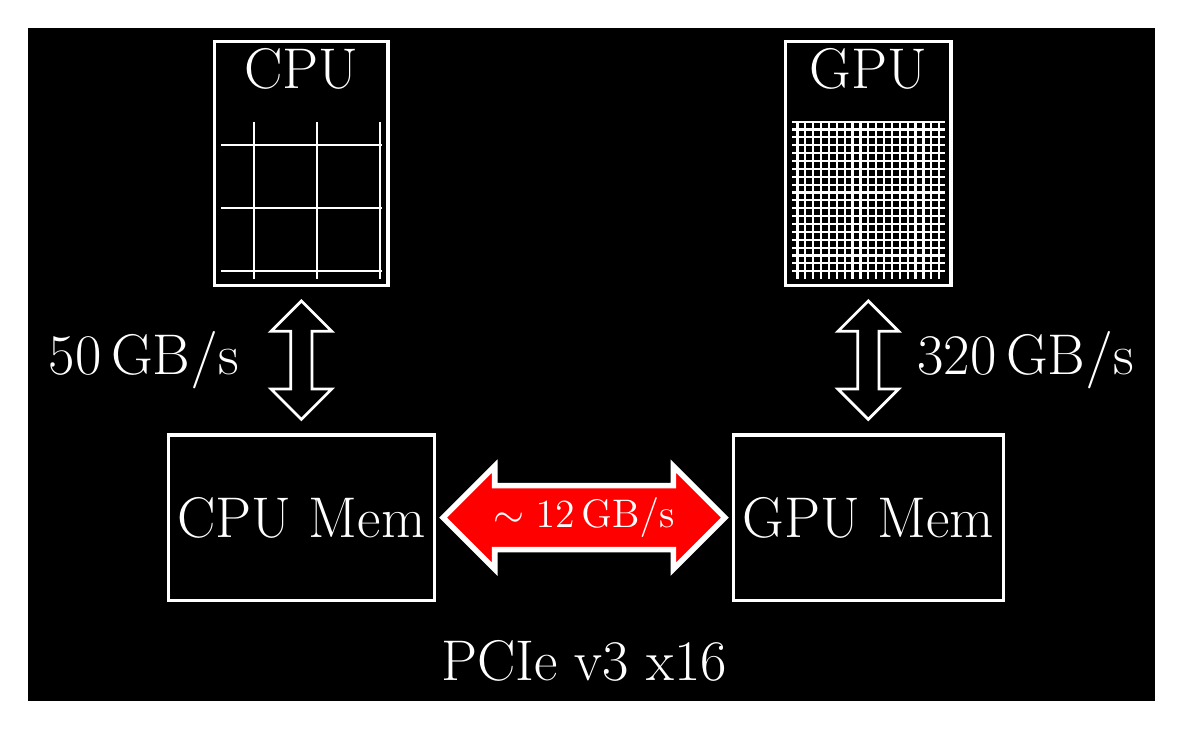
\begin{tikzpicture}[
  show background rectangle, 
  background rectangle/.style={fill=black},
  color=white,
  help lines/.style={color=lightgray,line width=.2pt},
  ]

  \node (cpu) [rectangle,minimum width=2.2cm,minimum height=3.1cm,very thick,draw=white,anchor=south] at(-0.2,-0.2) {};
  \node (cpu_name) [font=\huge,draw=none,below] at(cpu.north) {CPU};
  \draw[thick,step=.8cm] ($(cpu.south west)+(.1,.1)$) grid ($(cpu.south east)+(-.1,2.1)$);

  \node (cpu_ram) [font=\huge,rectangle,minimum width=3.1cm,minimum height=2.1cm,very thick,draw=white,anchor=south] at($(cpu.south)-(0,4)$) {CPU Mem};

  \node (gpu) [rectangle,minimum width=2.1cm,minimum height=3.1cm,very thick,draw=white,anchor=south] at(7,-.2) {};
  \node (gpu_name) [font=\huge,draw=none,below] at(gpu.north) {GPU};
  \draw[thick,step=.1cm] ($(gpu.south west)+(.1,.1)$) grid ($(gpu.south east)+(-.1,2.1)$);

  \node (gpu_ram) [font=\huge,rectangle,minimum width=3.1cm,minimum height=2.1cm,very thick,draw=white,anchor=south] at($(gpu.south)-(0,4)$) {GPU Mem};

  \node (PCIexpress_arrow) [double arrow, draw=white,fill=red, line width=2pt,font=\Large,inner xsep=.2cm] at($(cpu_ram.east)!.5!(gpu_ram.west)$) {$\sim\unit[12]{GB/s}$};
  \node (PCIexpress_name) [draw=none,font=\huge,below=1cm] at(PCIexpress_arrow.south) {PCIe v3 x16};

  \node (gpumem_arrow) [double arrow, draw, line width=1pt,inner xsep=.6cm,font=\Large,rotate=-90] at($(gpu.south)!.5!(gpu_ram.north)$) {};
  \node (gpumem_name) [draw=none,font=\huge] at($(gpu.south)!.5!(gpu_ram.north) + (2,0)$) {$\unit[320]{GB/s}$};

  \node (cpumem_arrow) [double arrow, draw, line width=1pt,inner xsep=.6cm,font=\Large,rotate=-90] at($(cpu.south)!.5!(cpu_ram.north)$) {};
  \node (cpumem_name) [draw=none,font=\huge] at($(cpu.south)!.5!(cpu_ram.north) + (-2,0)$) {$\unit[50]{GB/s}$};

% %  \draw[dashed, very thick] (5,-1) rectangle (25,14) ;
%   \foreach \c in {0,...,3}
%   {
%     %\draw[-] ($(0.2,2.05)+(2.4*\c,0)$) rectangle ($(2.3,2.75)+(2.4*\c,0)$) node[fitting node] (l2_\c) {\bfseries{}L2};
%     \node (smx_\c) [very thick,draw,rectangle, minimum width=3cm, minimum height=4cm,font=\huge] at($(8,10)+(3.5*\c,0)$) {};
%     \node [very thick,font=\huge,anchor=north] at(smx_\c.north) {\bfseries{}SMX};
%     \node (smx_\c_topright) [below =of smx_\c.north east] {};
%     \draw[step=.2] (smx_\c.south west) grid (smx_\c_topright);
%   }

%   \foreach \i in {0,...,4}
%   \draw[-latex,very thick] ($(8,6)+(3.5*\i,0)$) -- ($(8,7.7)+(3.5*\i,0)$) 
%   ;
  
%   \node (dots) [text=white,font=\huge] at($(8,10)+(14,0)$) {\bfseries{}\dots};

%   \draw[very thick] ($(8,6)$) -- ($(8,6)+(3.5*4,0)$) ;

%   \node (l2cache) [very thick,draw,rectangle, minimum width=12cm, minimum height=2cm,font=\Huge] at($(8,10)+(7,-6)$) {\bfseries{}GPU L2 Cache};
%   \node (dram) [very thick,draw,rectangle, minimum width=12cm, minimum height=2cm,font=\Huge] at($(8,10)+(7,-9)$) {\bfseries{}GPU DRAM};

%   \node (cpu_ram) [very thick,draw,rectangle, minimum width=4.5cm, minimum height=12cm,font=\Huge] at($(0,10)+(0,-4)$) {\bfseries{}CPU RAM};

%   % \draw[ultra thick] (cpu_ram) -- (dram);
  
%   %\draw[|<->|,very thick,double equal sign distance, line width=1mm, double distance=1.5mm,-Stealth] (dram.west) -- (cpu_ram.east);
%   \node (middle) at($(dram.west)+(-3.2,0)$) {};
%   \node [double arrow, draw, line width=1pt,font=\huge,inner xsep=.6cm,inner ysep=.3cm] at(middle) {PIC Express};
%   \draw[ultra thick] (l2cache.south) -- (dram.north);


%   \draw[very thick] (dram) -- (l2cache);
%   \draw[very thick] (l2cache) -- ($(8,6)+(7,0)$);
  

\end{tikzpicture}
\end{document}
